% !TeX spellcheck = ca
\documentclass{article}
\usepackage[utf8]{inputenc}
\usepackage{amsmath}
\usepackage{ amssymb }
\usepackage{float}
\usepackage{subfiles}
\usepackage{listings}
\usepackage{graphicx}

%Tot això hauria d'anar en un pkg, però no sé com és fa
\newcommand*{\assignatura}[1]{\gdef\1assignatura{#1}}
\newcommand*{\grup}[1]{\gdef\3grup{#1}}
\newcommand*{\professorat}[1]{\gdef\4professorat{#1}}
\renewcommand{\title}[1]{\gdef\5title{#1}}
\renewcommand{\author}[1]{\gdef\6author{#1}}
\renewcommand{\date}[1]{\gdef\7date{#1}}
\renewcommand{\baselinestretch}{1.5}
\renewcommand{\maketitle}{ %fa el maketitle de nou
	\begin{titlepage}
		\raggedright{UNIVERSITAT DE LLEIDA \\
			Escola Politècnica Superior \\
			Grau en Enginyeria Informàtica\\
			\1assignatura\\}
		\vspace{5cm}
		\centering\huge{\5title \\}
		\vspace{3cm}
		\large{\6author} \\
		\normalsize{\3grup}
		\vfill
		Professorat : \4professorat \\
		Data : \7date
\end{titlepage}}
%Emplenar a partir d'aquí per a fer el títol : no se com es fa el package
%S'han de renombrar totes, inclús date, si un camp es deixa en blanc no apareix


\title{Complete Sat Report}
\author{Joaquim Pico Mora, Ian Palacín Aliana}
\date{Divendres 28 Maig}
\assignatura{Programació avançada en intel·ligència artificial}
\professorat{Josep Argelich Roma}
\grup{}

\renewcommand{\refname}{Bibliografia}

%Comença el document
\begin{document}
	\maketitle
	\thispagestyle{empty}


%Fer intro?
\section{Introduction}
%Chachareria per omplir.
\section{Complete Sat}
%
\subsection{Skeleton}
%
\subsection{Heuristics}
In this section we're gonna pass trough all the heuristics explaining how had been implemented and also we're going to discuss the results that they have given to us. 
\subsubsection{Most Ocurrences}
Firstly we have the most ocurrences heuristic. As his name says, the literal that we pick to propagate is the one that apears the most in the formula. In orther to get it, we iterate trough the clauses and literals acounting all the ocurrences of each literal and latter geting the one that apers the most.
\subsubsection{Most Ocurrences in Minimum Size}
This heuristic gets the literal that appears the most in a minimum clause size. After unit propagation, the minimum size a clause can have is 2 literals, so most of the time we will start with size 2. Another thing to consider is that if there is a tie between two literals or more, we have to break the tie loking for the apparences of those literals in the clauses with one literal more, and if there is another tie with some of them, we have to look for one more...\\
In orther to do this, we get the minimum size of the clauses in the formula after the unit propagation and then we get the clauses with that size. After that we count the apparences of the litterals in the clauses get the one the appeared the most. In case of having a tie, we have a function called tiebraker that repeats the same for bigger clauses until it gets the final litteral.
\subsubsection{Most Equilibrated}
This one takes into acount the aparences of the litteral and the negated litteral, counting the times that apear each one of them. After geting the result, it multiplies the apparences of the litteral and the apparences of the negated literal and gets the one that results with the bigest number. This means that is the most equilibrated and is the one that we have to choose to propagate.\\
In orther to implement it, we used the same strategy that in the most ocurrences heuristic, but this time  instead of counting each literal separetly we count each symbol geting the times that apear positive and negated.
\subsubsection{Jeroslow Wang}
%
Jeroslow Wang take into account all the ocurrences of the literals in the formula, making the apparences of literals in small clauses have more importance due to the formula  $\sum 2^{-len(c)}$. We can see that as smaller is the length of the clause better.
In orther to do it we iterate through the formula and we make the sumatorium of the occurences of all the litterals. The one that results with the bigust value is the one that we pick. 
\subsubsection{Jeroslow Wang Two Sided}
%
This is a interesting implementation of Jeroslow Wang that we find that takes into the sumatorium of each literal takes into acount the negated literal too. It's implemented the same way as normal Jeroslow Wang, but acounting all the apparences of a symbol.
\subsubsection{Results}
% Gràfics% Comentar resultats
The graphic that we provide next has been made with the results of executing each heuristic with random 3 cnfs formulas of 75 variables and with a variable number of clauses(X axys). Each formula have been executed 25 times per heuristic and we made the mean in orther to get the resulting value of time(Y axys).   
\begin{figure}[H]
  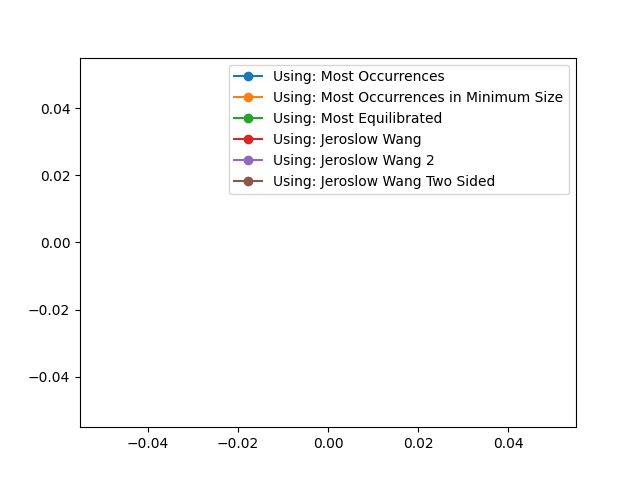
\includegraphics[width=\linewidth]{../utils/plots/heuristics.png}
  \caption{Heuristics comparation.}
  \label{fig:heu}
\end{figure}
In this plot \ref{fig:heu} we can see that the fastest heuristic is the 2 sided Jeroslow Wang. Surprisingly it performs really well, even Jeroslow Wang is not one of the best heuristics as we can see in the plot, it doesn't take care of the same symblol negated literals. Contempling this literals into Jeroslow Wang does not add more complexity in time and as we can see it makes it perform the way better.
The badest heuristic but not for that much is most occurences, which makes sence but is probably the least informed one. 
From the rest, we can see that more or less perform the same way but we can highlight that MOMS heuristic seems to perform better with hard formulas and don't have huge peaks at all.
\section{Python improvements}
%
\section{Profiling}
%
As we wanted to optimize the sat, we made a profiling using cProfile in orther to know wich of the functions were the ones that the algorithm executes the most and the ones in wich spends most of the time. Doing this has hepled us to optimize and improve the code in those critical points of the agorithm.
\section{Conclusions}
%Chachareria per omplir
\end{document}